\section{Theorie}
\label{sec:Theorie}

Ein Gerät, welches eine konstante Leistung über
einen endlichen Zeitraum erzeugen kann, beschreibt eine Spannungsquelle. Es wird von einer Leerlaufspannung $ U_0 $
an den Ausgangsklemmen gesprochen, falls der Spannungsquelle kein Strom entnommen wird.
Sobald es zu einer Leistungsabnahme durch einen äußeren Widerstand $ R_a $ kommt,
sinkt die an den Klemmen gemessene Spannung, die "Klemmenspannung", unter den Wert von $ U_0 $. Erklärt wird
dies durch einen Eigenwiderstand der Spannungsquelle. In der Theorie wird die reale
Spannungsquelle durch eine ideale Spannungsquelle in Reihe mit einem Widerstand $ R_i$
ersetzt.
\begin{figure}[H]
  \centering

  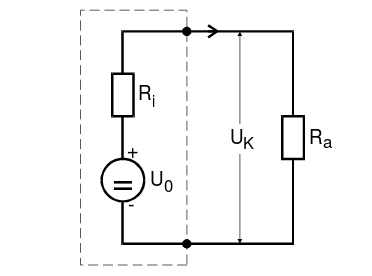
\includegraphics[width=\linewidth-200pt,height=\textheight-200pt,keepaspectratio]{content/Spannungsquelle1.png}
  \caption{Reale Spannungsquelle}
  \label{fig:Spannung1}
\end{figure}

Aus dem zweiten kirchhoffschen Gesetz folgt dann gemäß Abb. 1
\begin{equation}
	 U_0 = I R_i + I R_a  \text{ bzw. } U_k = I R_a = U_0-IR_i
\end{equation}
Zur Messung der Leerlaufspannung wird deshalb ein hochohmiges Voltmeter verwendet,
sodass der Strom $sI$ gegen $0$ läuft und somit $U_0 \approx U_k$ gilt.\\
\\
Aufgrund von $R_i$ kann der Spannungsquelle auch keine beliebig hohe Leistung
entnommen werden.Sie ergibt sich mit
\begin{equation}
  N = I^2 R_a
  \end{equation}
  und
\begin{equation}
   I =\frac{U_0}{R_a R_i}\text{.}
 \end{equation}
  Es lässt sich erkennen das $I(R_a)$
  ein Maximum besitz. Wird dieses erreicht, wird von Leistungsanpassung gesprochen.
